\documentclass[a4paper]{article}

\usepackage{amsmath}
\usepackage{hyperref}
\usepackage{biblatex}
\usepackage{enumerate}
\usepackage{graphicx}
\usepackage{stmaryrd}
\usepackage[dvipsnames]{xcolor}
\usepackage{listings}
\usepackage{float}
\addbibresource{refs.bib}

\begin{document}

\author{
  Sebastian Miles \\
  \href{mailto:miless@chalmers.se}{miless@chalmers.se}
  \and
  Olle Lapidus \\
  \href{mailto:ollelap@chalmers.se}{ollelap@chalmers.se}
}
\title{DAT565/DIT407 Assignment 1}
\date{2024-09-06}

\maketitle

\section*{Problem 1}
The goal of this assignment is to analyze the data downloaded from SCB~\cite{SCB:2023}. The data contains the number of people in Sweden by age and sex from 1860 to 2022. 
\subsection*{Task I}
The first task is to calculate the Dependency ratio of Sweden from 1860 to 2022. The dependency ratio is calculated as
\begin{align*}
\text{Dependency Ration } &= 100\cdot \frac{\text{\#children}+\text{\#elderly}}{\text{\#labor force}}\\
&= 100\cdot \frac{\text{\#people aged 0-14}+\text{\#people aged 65-}}{\text{\#people aged 15-64}}.
\end{align*}
The result can be viewed in Figure \ref{fig:depenratio}.
\begin{figure}[H]
  \begin{center}
    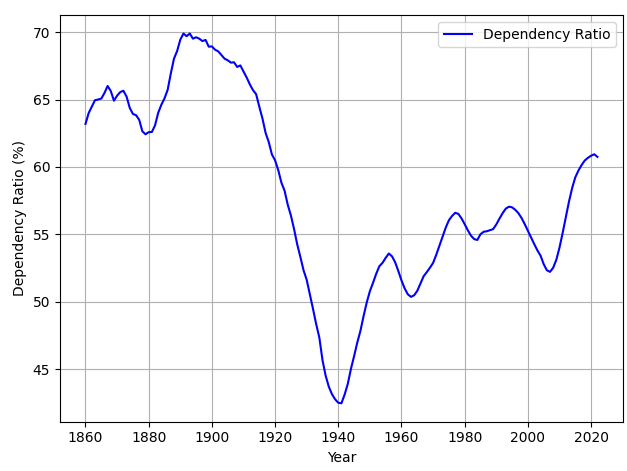
\includegraphics[scale=0.5]{depenratio.png}
    \caption{Dependency Ratio Over Time in Sweden (1860-2022)}
    \label{fig:depenratio}
  \end{center}
\end{figure}

\subsection*{Task II}
In this task we calculate the ratio of children, workforce and elderly respectively and plot it using the same data as before.
The result is show in Figure \ref{fig:frac}.



\begin{figure}[H]
  \begin{center}
    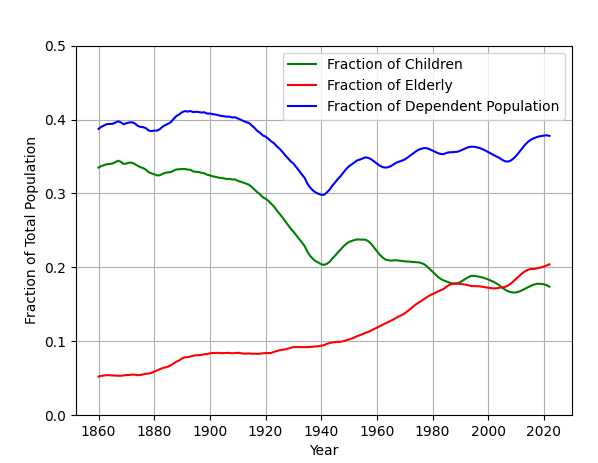
\includegraphics[scale=0.5]{frac.png}
    \caption{Fractions of Children, Elderly, and Total Dependent Population  in Sweden (1860-2022).}
    \label{fig:frac}
  \end{center}
\end{figure}

\subsection*{Task III}
Here we discuss the development of the Swedish population by observing Figure \ref{fig:depenratio} and Figure \ref{fig:frac}.
With advancements within the medical field and improved living conditions, people tend to live longer. It is therefore natural for the fraction of elderly to increase. The fraction of children has decreased because of better access to contraceptive devices, higher costs of raising children and drifting societal values towards having smaller families. World War I and II caused both societal and economical changes which also made it less appealing to have children which is clearly reflected in both figures above roughly in the years 1910-1940.\\


\printbibliography
\appendix

\section*{Code}
\label{app:code}

\lstset{
	language=Python,
	basicstyle=\ttfamily,
	commentstyle=\color{OliveGreen},
	keywordstyle=\bfseries\color{Magenta},
	stringstyle=\color{YellowOrange},
	numbers=left,
	frame=tblr,
	breaklines=true,
	postbreak=\mbox{\textcolor{red}{$\hookrightarrow$}\space},
}
\begin{lstlisting}
import pandas as pd
import matplotlib.pyplot as plt

# Read from file
df = pd.read_csv('swedish_population_by_year_and_sex_1860-2022.csv')


# Cast age column to integer
df['age'] = pd.to_numeric(df['age'], errors='coerce')

# Extract age groups
children = df[df['age'] <= 14]
workforce = df[(df['age'] > 14) & (df['age'] <= 64)]
elderly = df[df['age'] > 64]

# Compute the group populations
total_children  = children[children.columns[2:]].sum()
total_workforce  = workforce[workforce.columns[2:]].sum()
total_elderly  = elderly[elderly.columns[2:]].sum()

dependency_ratio = 100*(total_children+total_elderly)/(total_workforce)

plt.plot(dependency_ratio.index, dependency_ratio.values, label='Dependency Ratio', color='b')
plt.xlabel('Year')
plt.ylabel('Dependency Ratio (%)')
plt.grid(True)
plt.legend()
plt.gca().xaxis.set_major_locator(plt.MaxNLocator(nbins=10))

plt.show()

# Compute the total population across all ages
total_population = total_children + total_workforce + total_elderly

# Compute the ratio of each group
ratio_children  = total_children/total_population
ratio_elderly  = total_elderly/total_population
ratio_dependent  = (total_elderly+total_children)/total_population

plt.plot(ratio_children.index, ratio_children.values, label='Fraction of Children', color='g')
plt.plot(ratio_elderly.index, ratio_elderly.values, label='Fraction of Elderly', color='r')
plt.plot(ratio_dependent.index, ratio_dependent.values, label='Fraction of Dependent Population', color='b')

plt.xlabel('Year')
plt.ylabel('Fraction of Total Population')
plt.ylim(0,0.5)
plt.grid(True)
plt.legend()
plt.gca().xaxis.set_major_locator(plt.MaxNLocator(nbins=10))

plt.show()

\end{lstlisting}

\end{document}
